\chapter{Flotar y hundirse}\label{ch:g1:floating-and-sinking}

Tira un guijarro a un charco: desaparece hasta el fondo. Tira una
hoja: viaja por encima como un barquito. La bañera, los charcos y los
estanques hacen todos la misma pregunta --- ¿qué \omterm{def:g1:floating-and-sinking:words}{flota}, qué
\omterm{def:g1:floating-and-sinking:words}{se hunde} y podemos adivinarlo antes de tirarlo al agua?

\section{¿Flota o se hunde?}

\begin{definition}[Flotar y hundirse]\label{def:g1:floating-and-sinking:words}
Una cosa \emph{flota}\index{flotar} cuando el agua la sujeta arriba,
en la superficie; \emph{se hunde}\index{hundirse} cuando baja hasta el
fondo. Un corcho flota; un guijarro se hunde.
\end{definition}

\begin{method}[Una prueba de flotación justa]\label{met:g1:floating-and-sinking:test}
\begin{enumerate}
  \item llena de agua un barreño grande (o el fregadero);
  \item posa el objeto sobre el agua con \emph{suavidad} --- nada de
        tirarlo: una salpicadura puede hundir un momento hasta lo que
        \omterm{def:g1:floating-and-sinking:words}{flota};
  \item suéltalo del todo y espera mientras cuentas hasta $5$;
  \item mira: arriba está lo que \omterm{def:g1:floating-and-sinking:words}{flota}, en el fondo está lo que \omterm{def:g1:floating-and-sinking:words}{se
        hunde}.
\end{enumerate}
Prueba cada objeto de la misma manera, para que la comparación sea
justa.
\end{method}

\begin{example}[Pruébalo: el juego de clasificar]\label{ex:g1:floating-and-sinking:sorting}
Reúne un corcho, una moneda, una cuchara de plástico, una cuchara de
metal, un guijarro, un lápiz y una hoja seca, y pruébalos uno a uno
con el \cref{met:g1:floating-and-sinking:test}. Flotan: el corcho, la
cuchara de plástico, el lápiz, la hoja. Se hunden: la moneda, la
cuchara de metal, el guijarro. Antes de soltar cada objeto, di en voz
alta lo que crees que va a pasar --- eso es lo que los científicos
llaman una \emph{predicción}, y equivocarse es la mitad de la
diversión.
\end{example}

\begin{omfigure}
\begin{tikzpicture}[scale=0.85]
  \draw[thick] (0,0) -- (0,3.2) (0,0) -- (9,0) (9,0) -- (9,3.2);
  \fill[omDef, opacity=0.15] (0,0) rectangle (9,2.6);
  % cork: a little cylinder riding half-sunk
  \draw[thick, fill=brown!45] (1.25,2.38) rectangle (1.75,2.78);
  \draw[thick, fill=brown!30] (1.5,2.78) ellipse (0.25 and 0.08);
  \node[above, font=\small] at (1.5,3.0) {corcho};
  % leaf: pointed oval with a midrib, flat on the surface
  \draw[thick, green!45!black, fill=green!40]
    (3.6,2.62) .. controls (4.0,2.92) and (4.5,2.92) .. (4.85,2.62)
    .. controls (4.5,2.52) and (4.0,2.52) .. (3.6,2.62);
  \draw[green!45!black] (3.68,2.63) -- (4.78,2.63);
  \draw[thick, green!45!black] (3.6,2.62) -- (3.42,2.56);
  \node[above, font=\small] at (4.2,3.0) {hoja};
  % pencil: yellow body, sharpened tip, lying on the water
  \draw[thick, fill=red!45] (5.95,2.56) rectangle (6.1,2.76);
  \draw[thick, fill=yellow!75] (6.1,2.56) rectangle (7.6,2.76);
  \draw[thick, fill=brown!35] (7.6,2.56) -- (7.95,2.66)
    -- (7.6,2.76) -- cycle;
  \fill[black] (7.95,2.66) -- (7.85,2.62) -- (7.85,2.7) -- cycle;
  \node[above, font=\small] at (6.9,3.0) {lápiz};
  % pebble: an irregular gray lump on the bottom
  \draw[thick, fill=omExo!55]
    (2.25,0.18) .. controls (2.3,0.45) and (2.75,0.52) .. (2.95,0.32)
    .. controls (3.05,0.18) and (2.9,0.04) .. (2.6,0.04)
    .. controls (2.4,0.04) and (2.25,0.06) .. (2.25,0.18);
  \node[above, font=\small] at (2.6,0.6) {guijarro};
  % coin: a flat golden disc
  \draw[thick, fill=yellow!70!orange] (5.15,0.04) rectangle (5.65,0.12);
  \draw[thick, fill=yellow!85!orange] (5.4,0.12) ellipse (0.25 and 0.07);
  \node[above, font=\small] at (5.4,0.45) {moneda};
  % metal spoon: bowl plus handle
  \draw[thick, fill=omExo!40] (7.05,0.2) ellipse (0.34 and 0.16);
  \draw[line width=2.4pt, omExo!80!black] (7.38,0.16) -- (8.5,0.08);
  \node[above, font=\small] at (7.8,0.55) {cuchara de metal};
  % the water in front of everything, and its surface line
  \fill[omDef, opacity=0.12] (0,0) rectangle (9,2.6);
  \draw[omDef, thick] (0,2.6) -- (9,2.6);
\end{tikzpicture}

{\small Después del juego de clasificar: lo que \omterm{def:g1:floating-and-sinking:words}{flota} viaja en la
superficie del agua, lo que \omterm{def:g1:floating-and-sinking:words}{se hunde} descansa en el fondo.}
\end{omfigure}

\begin{omfigure}
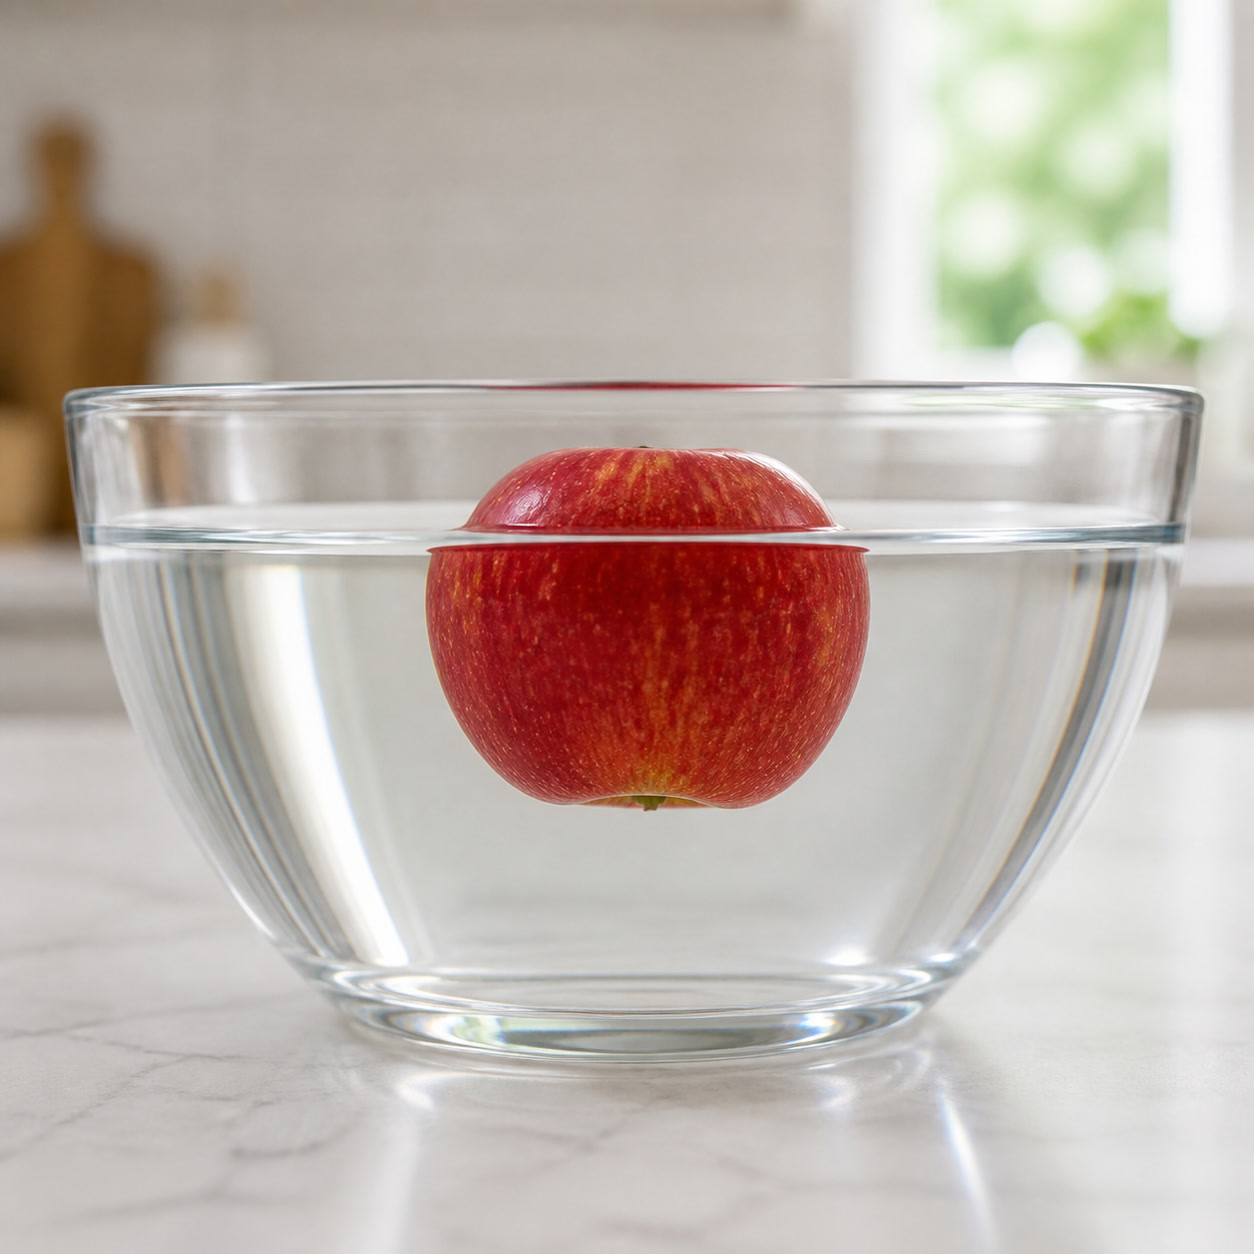
\includegraphics[width=0.42\linewidth]{images/book1/ai/g1-floating-apple.jpg}

{\small Una manzana flotando en un cuenco de agua: va muy baja, con casi todo el cuerpo por debajo de la superficie --- y aun así \omterm{def:g1:floating-and-sinking:words}{flota}.}
\end{omfigure}

\section{Ser pesado no lo explica todo}

Mucha gente supone que ``las cosas pesadas se hunden y las ligeras
flotan''. El agua les tiene guardada una sorpresa.

\begin{example}[El tronco y la moneda]\label{ex:g1:floating-and-sinking:log}
Un tronco caído pesa muchísimo más de lo que tú puedes levantar --- y
sin embargo \omterm{def:g1:floating-and-sinking:words}{flota} río abajo. Una moneda pequeña pesa menos que una
galleta --- y sin embargo \omterm{def:g1:floating-and-sinking:words}{se hunde} enseguida. Así que ser pesado o
ligero no puede ser toda la regla: el tronco enorme \omterm{def:g1:floating-and-sinking:words}{flota} mientras
la monedita se va al fondo.
\end{example}

\begin{example}[Lo que cuenta es el material]\label{ex:g1:floating-and-sinking:stuff}
Vuelve al juego de clasificar: la cuchara de plástico flotó y la de
metal se hundió, aunque tienen la misma forma y sirven para lo mismo.
Lo que marcó la diferencia es el \emph{material} del que están hechas
--- la madera, el corcho y casi todos los plásticos son materiales que
flotan; el metal, la piedra y el vidrio son materiales que se hunden.
Una cosa se comporta casi siempre como su material: la madera \omterm{def:g1:floating-and-sinking:words}{flota}
lo mismo si es una ramita que si es un tronco entero.
\end{example}

\begin{remark}[Una pizca de misterio]\label{rem:g1:floating-and-sinking:why}
¿Y \emph{por qué} la madera \omterm{def:g1:floating-and-sinking:words}{flota} y el metal \omterm{def:g1:floating-and-sinking:words}{se hunde}? Esa es una
buena pregunta, y su respuesta completa es uno de los tesoros de este
curso --- necesita ideas que llegan en años posteriores. Por ahora
recogemos buenas observaciones; el ``porqué'' nos encontrará
preparados.
\end{remark}

\section{El agua empuja hacia arriba}

\begin{example}[Pruébalo: hunde la pelota]\label{ex:g1:floating-and-sinking:push}
Coge una pelota que flote en la bañera y húndela despacio con la palma
de la mano. ¿Lo notas? El agua la empuja hacia arriba, y con más
fuerza cuanto más hondo la metes --- y si se te escapa la mano, la
pelota salta fuera del agua. El agua no se limita a \emph{dejar} que
las cosas se queden encima: las sujeta activamente, como unos brazos
que sostienen a un bebé.
\end{example}

\begin{omfigure}
\begin{tikzpicture}[scale=0.85]
  \draw[thick] (0,0) -- (0,3.4) (0,0) -- (6.5,0) (6.5,0) -- (6.5,3.4);
  \draw[omDef, thick] (0,2.7) -- (6.5,2.7);
  \fill[omDef, opacity=0.15] (0,0) rectangle (6.5,2.7);
  \draw[thick, fill=white] (3.2,1.5) circle (0.6);
  \node[font=\small] at (3.2,1.5) {pelota};
  \draw[-Stealth, very thick, omThm] (3.2,3.3) -- (3.2,2.25);
  \node[right, font=\small, omThm] at (3.35,2.9) {tu mano empuja hacia abajo};
  \draw[-Stealth, very thick, omDef] (3.2,0.35) -- (3.2,0.85);
  \node[right, font=\small, omDef] at (3.35,0.55) {el agua empuja hacia arriba};
\end{tikzpicture}

{\small Una pelota sujeta bajo el agua: tu mano empuja hacia abajo, el
agua empuja hacia arriba. Suéltala y gana el empuje del agua.}
\end{omfigure}

\begin{example}[El barco de plastilina]\label{ex:g1:floating-and-sinking:boat}
Haz una bola con un trozo de plastilina y échala al agua: \omterm{def:g1:floating-and-sinking:words}{se hunde}
--- la plastilina es un material que \omterm{def:g1:floating-and-sinking:words}{se hunde}. Coge ahora el
\emph{mismo} trozo, dale forma de cuenco con las paredes altas y
pósalo con suavidad sobre el agua: ¡\omterm{def:g1:floating-and-sinking:words}{flota}! Mismo material, mismo
trozo --- lo único que ha cambiado es la forma. Una forma ancha y
hueca le da al agua más superficie sobre la que empujar. Ese es el
secreto de los grandes barcos: el metal es un material que \omterm{def:g1:floating-and-sinking:words}{se hunde},
pero un casco de metal tiene forma de cuenco hueco enorme.
\end{example}

\begin{omfigure}
\begin{tikzpicture}[scale=0.85]
  \draw[thick] (0,0) -- (0,2.6) (0,0) -- (4.6,0) (4.6,0) -- (4.6,2.6);
  \draw[omDef, thick] (0,2.0) -- (4.6,2.0);
  \fill[omDef, opacity=0.15] (0,0) rectangle (4.6,2.0);
  \fill[omThm] (2.3,0.35) circle (0.35);
  \node[below, font=\small] at (2.3,-0.2) {bola de plastilina: se hunde};
  \draw[thick] (6.4,0) -- (6.4,2.6) (6.4,0) -- (11,0)
    (11,0) -- (11,2.6);
  \draw[omDef, thick] (6.4,2.0) -- (11,2.0);
  \fill[omDef, opacity=0.15] (6.4,0) rectangle (11,2.0);
  \draw[thick, omThm, fill=white]
    (7.9,2.25) -- (8.1,1.75) -- (9.3,1.75) -- (9.5,2.25);
  \node[below, font=\small] at (8.7,-0.2) {el mismo trozo en cuenco: flota};
\end{tikzpicture}

{\small Un trozo de plastilina, dos formas, dos destinos. La forma
hueca de cuenco le da al agua más superficie que sostener.}
\end{omfigure}

\section{Ejercicios}

\begin{exercise}[$\star$]\label{exo:g1:floating-and-sinking:1}
Separa en cosas que flotan y cosas que se hunden: un corcho; \ una
llave; \ una ramita seca; \ una canica; \ un patito de plástico; \ una
piedra.
\end{exercise}

\begin{exercise}[$\star$]\label{exo:g1:floating-and-sinking:2}
En el \cref{met:g1:floating-and-sinking:test}, ¿por qué hay que posar
el objeto sobre el agua con suavidad en vez de tirarlo?
\end{exercise}

\begin{exercise}[$\star$]\label{exo:g1:floating-and-sinking:3}
Antes de la prueba, Nora supone: ``La cuchara de metal flotará
porque las cucharas flotan''. ¿Qué pasó en el juego de clasificar?
¿En qué debería fijarse Nora en vez de fijarse en para qué sirve la
forma: en el material o en el nombre?
\end{exercise}

\begin{exercise}[$\star$]\label{exo:g1:floating-and-sinking:4}
Di una cosa que sea pesada y flote, y una cosa que sea ligera y
se hunda. ¿Qué demuestra esto sobre la suposición ``las cosas
pesadas se hunden''?
\end{exercise}

\begin{exercise}[$\star$]\label{exo:g1:floating-and-sinking:5}
Una ramita \omterm{def:g1:floating-and-sinking:words}{flota}. ¿Flotará también un tronco entero? ¿Qué
ejemplo del capítulo te ayuda a responder?
\end{exercise}

\begin{exercise}[$\star$]\label{exo:g1:floating-and-sinking:6}
Hunde en la bañera una pelota que flote y suéltala. ¿Qué notas
mientras la empujas y qué hace la pelota cuando la sueltas?
\end{exercise}

\begin{exercise}[$\star$]\label{exo:g1:floating-and-sinking:7}
Los barcos están hechos de metal, y el metal es un material que \omterm{def:g1:floating-and-sinking:words}{se
hunde}. ¿Qué forma salva al barco? ¿Qué experimento del capítulo lo
demuestra?
\end{exercise}

\begin{exercise}[$\star$]\label{exo:g1:floating-and-sinking:8}
Prueba a la hora del baño: una botella llena de agua y cerrada,
¿\omterm{def:g1:floating-and-sinking:words}{flota} o \omterm{def:g1:floating-and-sinking:words}{se hunde}? ¿Y la misma botella vacía, con el tapón
puesto? Di primero lo que crees y pruébalo después.
\end{exercise}

\begin{exercise}[$\star\star$]\label{exo:g1:floating-and-sinking:9}
El barco de plastilina de Leo \omterm{def:g1:floating-and-sinking:words}{flota} estupendamente --- hasta que lo
aplasta y lo deja hecho una bola, y entonces \omterm{def:g1:floating-and-sinking:words}{se hunde}. ``El agua se
ha cansado de sujetarlo'', dice Leo. Da una explicación mejor, usando
el \cref{ex:g1:floating-and-sinking:boat}.
\end{exercise}
